\section{TopoGen Dataset}
\label{sec:topogen}

Assessing how models understand the topology of 3D shapes, in particular through probing, requires data labeled with topological information and control over the distribution of the labels. However such dataset, specifically designed with a focus on the structure and not the semantics, hasn't been developed yet. Hence we introduce TopoGen, a scalable dataset of 3D synthetic shapes with accurate and well balanced topological labels. The samples in this dataset are labeled by number of connected components and genus.

\subsection{Existing datasets}
\label{ssec:existing_datasets}

When speaking about structural understanding, representations such as the ones present in the MANTRA \cite{mantra} dataset are a natural choice. The MANTRA dataset (Manifold Triangulation Assemblage) by Ballester et al. consists purely of combinatorial triangulation of 2- and 3-dimensional manifolds: i.e., its samples only include connectivity information (abstract simplicial complexes), without any geometric embedding in $\mathbb{R}^3$, making it agnostic to geometric realization. This makes MANTRA a particularly meaningful benchmark when assessing whether graph-based and simplicial complex-based models capture higher-order structures (essentially Betti numbers $\beta_0, \beta_1, \beta_2$ and $\beta_3$). However, in this work we focus on evaluating models that rely on geometric 3D representations such as meshes, point clouds, or implicit fields (e.g., Signed Distance Functions (SDFs)) (i.e., data embedded in $\mathbb{R}^3$. Therefore, MANTRA falls outside the scope of the tasks considered in this report.


Only a few large datasets have some considerations about structural information carried by meshes (commonly the number of connected components and the genus). Notably, the Thingi10K and ABC datasets, which are composed with various CAD models and artistic meshes come with such annotations. However, they turn out to be inaccurate for three reasons. 
\begin{enumerate}
  \item \textbf{Discrepancy between actual and effective number of components.} In artistic 3D modeling, a complex shape is often constructed from many mesh objects that represent fine details (buttons, ornaments, small extrusions, etc.). As a result, the true number of connected components in the mesh (counting every individual object used in the construction) can be much larger than the effective number of connected components, which corresponds to the main perceived object as a whole. (*+fig*). The same issue holds with complex CAD models.
  \item \textbf{Imbalanced annotations.} While both Thingi10K and ABC exhibit a wide range of genus values (Figure \ref{fig:thingi-genus} ADD FOR ABC), the distribution is highly imbalanced. For evaluation tasks such as probing, balanced annotations are crucial, yet in this dataset the vast majority of samples have very low genus (typically between 0 and 2), whereas high-genus shapes are severely underrepresented.
  \item \textbf{Structural artifacts.} Most meshes in these datasets are not suitable out-of-the-box for topological labelling. Many of them are non-manifold or contain self-intersecting faces. This raises two main issues. First, it makes topological analysis unreliable: for example, the Euler Characteristic (Equation \ref{eq:euler}) cannot be applied to non-manifold meshes.
\end{enumerate}
\begin{equation}
  \chi = V - E + F = 2 - 2g - b + c
  \label{eq:euler}
\end{equation}
Where $V, E, F$ are the number of vertices, edges and faces respectively, $g$ is the genus, $b$ the number of boundary components and $c$ the number of connected components.

\begin{figure}[t]
  \centering
  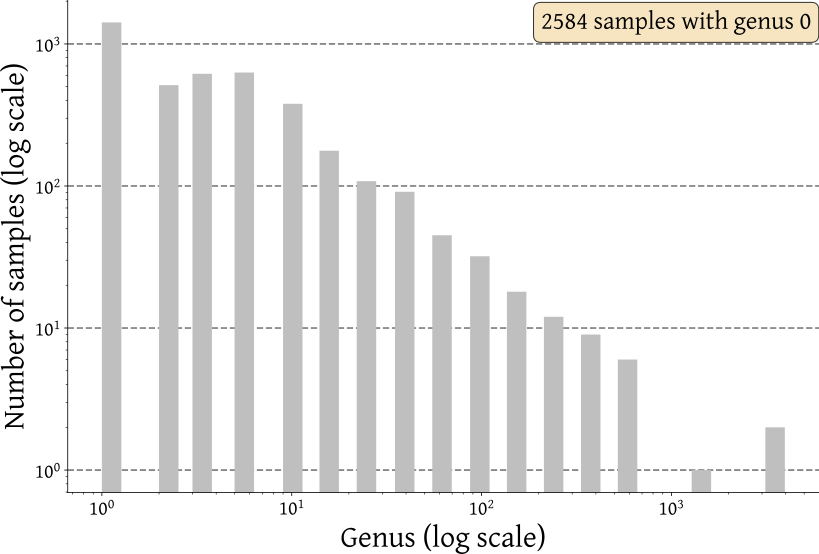
\includegraphics[width=\linewidth]{figs/topogen/thingi_genus_hist.pdf}
   \caption{\textbf{Genus distribution of Thingi10K.} Both axes are plotted in log scale. The genus was estimated from the Euler characteristic, provided as metadata with the dataset; however, 2,651 samples do not fulfill the requirements to directly compute the genus from the Euler characteristic (see \ref{eq:euler}). They are therefore not taken into account here. The histogram shows that a large fraction of the dataset (over 3,000 samples out of 7,344) has genera of 0 or 1, indicating that higher-genus components are significantly underrepresented, which may limit accurate classification and probing analyses for those cases.}
   \label{fig:thingi-genus}
\end{figure}


Second, self-intersections may introduce undesired topological structures, leading to inaccurate labels. To overcome these issues, remeshing procedures such as Manifold \cite{manifold} and ManifoldPlus \cite{manifoldplus} were proposed, transforming arbitrary meshes into manifold and watertight representations. While Manifold provides robustness, it often over smooths the input geometry, reducing fine details. ManifoldPlus improves accuracy but introduces artifacts (see Fig...) (*+example with flower pot*) in challenging cases, leading to inconsistencies in the resulting topology. More recent approaches rely on intermediate representations such as signed or unsigned distance fields. Methods like Dual Octree Graph Networks (DOGN) \cite{dogn}, and the remeshing procedure in CLAY \cite{clay} achieve more stable and reliable results, but at the cost of significantly higher computational complexity. Finally, some shapes in Thingi10K and ABC also exhibit highly uneven geometric complexity, which can negatively impact model evaluation. To ensure that results primarily reflect the topology of the shapes, a certain level of uniformity in geometric complexity across the dataset is necessary. However, quantifying geometric difficulty is challenging, as no straightforward metric exists to assess it. Moreover, since the shapes were not generated under a controlled process, it is not possible to design a general heuristic to filter out geometrically challenging samples consistently.


% Finally, the EuLearn dataset (Figure \ref{fig:eulearn-samples}), intended to supervise models on inferring the genus from point clouds, offers interesting perspectives to train on synthetic data. The dataset is generated from Fourier curves with additional procedures to create knots, which in turn produce surfaces of different genera and some topological diversity. Despite its scalability in terms of the number of samples, EuLearn only covers genera between 0 and 10. Moreover, the generation rules lead to very limited variation within each genus: samples of the same class tend to look too similar, which results in strong overfitting. @fig:eulearn_umap_aug and @tab:eulearn_overfit highlight this issue at the transformer features level while @fig:eulearn_samples and @fig:eulearn_acc_angle confirm this issue at the sample level. In particular, @fig:eulearn_acc_angle exhibits a strong correlation between shapes genera and their canonical orientation. Indeed, a simple nearest neighbors classifier with Chamfer distance achieves perfect accuracy on the test set if it's fit on the training set as is. Beyond this rotation-genus correlation, @fig:eulearn_face_to_vertex_ratio further shows that the geometric complexity (as measured by the face-to-vertex ratio) is strongly correlated with the genus. This correlation makes it difficult to disentangle whether classification performance is driven by topological information or by correlated geometric cues. Overall, these limitations make EuLearn unsuitable for robustly probing structural understanding in 3D shape encoders.

\begin{figure}[t]
  \centering
  \includegraphics[width=\linewidth]{figs/topogen/eulearn_samples.pdf}
   \caption{\textbf{Samples from the EuLearn dataset across different genera.} As the genus increases, shapes become geometrically more complex. This trend highlights a confounding factor in the dataset: geometric complexity grows together with genus. As a result, classification performance may be driven not only by topological information but also by correlated geometric cues.}
   \label{fig:eulearn-samples}
\end{figure}

% All text must be in a two-column format.
% The total allowable size of the text area is $6\frac78$ inches (17.46 cm) wide by $8\frac78$ inches (22.54 cm) high.
% Columns are to be $3\frac14$ inches (8.25 cm) wide, with a $\frac{5}{16}$ inch (0.8 cm) space between them.
% The main title (on the first page) should begin 1 inch (2.54 cm) from the top edge of the page.
% The second and following pages should begin 1 inch (2.54 cm) from the top edge.
% On all pages, the bottom margin should be $1\frac{1}{8}$ inches (2.86 cm) from the bottom edge of the page for $8.5 \times 11$-inch paper;
% for A4 paper, approximately $1\frac{5}{8}$ inches (4.13 cm) from the bottom edge of the
% page.

% %-------------------------------------------------------------------------
% \subsection{Margins and page numbering}

% All printed material, including text, illustrations, and charts, must be kept
% within a print area $6\frac{7}{8}$ inches (17.46 cm) wide by $8\frac{7}{8}$ inches (22.54 cm)
% high.
% %
% Page numbers should be in the footer, centered and $\frac{3}{4}$ inches from the bottom of the page.
% The review version should have page numbers, yet the final version submitted as camera ready should not show any page numbers.
% The \LaTeX\ template takes care of this when used properly.



% %-------------------------------------------------------------------------
% \subsection{Type style and fonts}

% Wherever Times is specified, Times Roman may also be used.
% If neither is available on your word processor, please use the font closest in
% appearance to Times to which you have access.

% MAIN TITLE.
% Center the title $1\frac{3}{8}$ inches (3.49 cm) from the top edge of the first page.
% The title should be in Times 14-point, boldface type.
% Capitalize the first letter of nouns, pronouns, verbs, adjectives, and adverbs;
% do not capitalize articles, coordinate conjunctions, or prepositions (unless the title begins with such a word).
% Leave two blank lines after the title.

% AUTHOR NAME(s) and AFFILIATION(s) are to be centered beneath the title
% and printed in Times 12-point, non-boldface type.
% This information is to be followed by two blank lines.

% The ABSTRACT and MAIN TEXT are to be in a two-column format.

% MAIN TEXT.
% Type main text in 10-point Times, single-spaced.
% Do NOT use double-spacing.
% All paragraphs should be indented 1 pica (approx.~$\frac{1}{6}$ inch or 0.422 cm).
% Make sure your text is fully justified---that is, flush left and flush right.
% Please do not place any additional blank lines between paragraphs.

% Figure and table captions should be 9-point Roman type as in \cref{fig:onecol,fig:short}.
% Short captions should be centred.

% \noindent Callouts should be 9-point Helvetica, non-boldface type.
% Initially capitalize only the first word of section titles and first-, second-, and third-order headings.

% FIRST-ORDER HEADINGS.
% (For example, {\large \bf 1. Introduction}) should be Times 12-point boldface, initially capitalized, flush left, with one blank line before, and one blank line after.

% SECOND-ORDER HEADINGS.
% (For example, { \bf 1.1. Database elements}) should be Times 11-point boldface, initially capitalized, flush left, with one blank line before, and one after.
% If you require a third-order heading (we discourage it), use 10-point Times, boldface, initially capitalized, flush left, preceded by one blank line, followed by a period and your text on the same line.

% %-------------------------------------------------------------------------
% \subsection{Footnotes}

% Please use footnotes\footnote{This is what a footnote looks like.
% It often distracts the reader from the main flow of the argument.} sparingly.
% Indeed, try to avoid footnotes altogether and include necessary peripheral observations in the text (within parentheses, if you prefer, as in this sentence).
% If you wish to use a footnote, place it at the bottom of the column on the page on which it is referenced.
% Use Times 8-point type, single-spaced.


% %-------------------------------------------------------------------------
% \subsection{Cross-references}

% For the benefit of author(s) and readers, please use the
% {\small\begin{verbatim}
%   \cref{...}
% \end{verbatim}}  command for cross-referencing to figures, tables, equations, or sections.
% This will automatically insert the appropriate label alongside the cross-reference as in this example:
% \begin{quotation}
%   To see how our method outperforms previous work, please see \cref{fig:onecol} and \cref{tab:example}.
%   It is also possible to refer to multiple targets as once, \eg~to \cref{fig:onecol,fig:short-a}.
%   You may also return to \cref{sec:formatting} or look at \cref{eq:also-important}.
% \end{quotation}
% If you do not wish to abbreviate the label, for example at the beginning of the sentence, you can use the
% {\small\begin{verbatim}
%   \Cref{...}
% \end{verbatim}}
% command. Here is an example:
% \begin{quotation}
%   \Cref{fig:onecol} is also quite important.
% \end{quotation}

% %-------------------------------------------------------------------------
% \subsection{References}

% List and number all bibliographical references in 9-point Times, single-spaced, at the end of your paper.
% When referenced in the text, enclose the citation number in square brackets, for
% example~\cite{Authors14}.
% Where appropriate, include page numbers and the name(s) of editors of referenced books.
% When you cite multiple papers at once, please make sure that you cite them in numerical order like this \cite{Alpher02,Alpher03,Alpher05,Authors14b,Authors14}.
% If you use the template as advised, this will be taken care of automatically.

% \begin{table}
%   \centering
%   \begin{tabular}{@{}lc@{}}
%     \toprule
%     Method & Frobnability \\
%     \midrule
%     Theirs & Frumpy \\
%     Yours & Frobbly \\
%     Ours & Makes one's heart Frob\\
%     \bottomrule
%   \end{tabular}
%   \caption{Results.   Ours is better.}
%   \label{tab:example}
% \end{table}

% %-------------------------------------------------------------------------
% \subsection{Illustrations, graphs, and photographs}

% All graphics should be centered.
% In \LaTeX, avoid using the \texttt{center} environment for this purpose, as this adds potentially unwanted whitespace.
% Instead use
% {\small\begin{verbatim}
%   \centering
% \end{verbatim}}
% at the beginning of your figure.
% Please ensure that any point you wish to make is resolvable in a printed copy of the paper.
% Resize fonts in figures to match the font in the body text, and choose line widths that render effectively in print.
% Readers (and reviewers), even of an electronic copy, may choose to print your paper in order to read it.
% You cannot insist that they do otherwise, and therefore must not assume that they can zoom in to see tiny details on a graphic.

% When placing figures in \LaTeX, it's almost always best to use \verb+\includegraphics+, and to specify the figure width as a multiple of the line width as in the example below
% {\small\begin{verbatim}
%    \usepackage{graphicx} ...
%    \includegraphics[width=0.8\linewidth]
%                    {myfile.pdf}
% \end{verbatim}
% }


% %-------------------------------------------------------------------------
% \subsection{Color}

% Please refer to the author guidelines on the \confName\ \confYear\ web page for a discussion of the use of color in your document.

% If you use color in your plots, please keep in mind that a significant subset of reviewers and readers may have a color vision deficiency; red-green blindness is the most frequent kind.
% Hence avoid relying only on color as the discriminative feature in plots (such as red \vs green lines), but add a second discriminative feature to ease disambiguation.